
%(BEGIN_QUESTION)
% Copyright 2009, Tony R. Kuphaldt, released under the Creative Commons Attribution License (v 1.0)
% This means you may do almost anything with this work of mine, so long as you give me proper credit

Determine what type of temperature sensor is shown in this pictorial diagram, and then sketch wires showing how to correctly connect the sensor to the temperature transmitter:

$$\includegraphics[width=15.5cm]{i03997x01.eps}$$

Note what types of metal each of the connecting wires should be (e.g. copper, chromel, alumel, constantan, iron, platinum, etc.).

\vskip 20pt \vbox{\hrule \hbox{\strut \vrule{} {\bf Suggestions for Socratic discussion} \vrule} \hrule}

\begin{itemize}
\item{} A problem-solving technique useful for making proper connections in pictorial circuit diagrams is to first identify the directions of all DC currents entering and exiting component terminals, as well as the respective voltage polarity marks (+,$-$) for those terminals, based on your knowledge of each component acting either as an electrical {\it source} or an electrical {\it load}.  Discuss and compare how these arrows and polarity marks simplify the task of properly connecting wires between components. 
\item{} Suppose the wire colors on the thermocouple were rubbed off, so you could not visually discern positive from negative.  A tag on the thermocouple still tells you the type, though.  Is there some other way we could determine thermocouple polarity?
\item{} Suppose all labels and wire colors on the thermocouple were rubbed off, so you could not even tell what kind of sensor it was: thermocouple, RTD, or thermistor.  Devise a simple test by which you could ascertain the identify of the temperature sensor.
\end{itemize}

\underbar{file i03997}
%(END_QUESTION)





%(BEGIN_ANSWER)

\noindent
{\bf Partial answer:}

\vskip 10pt

The sensor is a type T thermocouple.

%(END_ANSWER)





%(BEGIN_NOTES)

$$\includegraphics[width=15.5cm]{i03997x02.eps}$$

Note: other possibilities for wiring the 4-20 mA ``loop'' circuit exist, but the direction of current needs to be the same as for this circuit.  No alternative wiring schemes exist for the thermocouple, though, except the option of using {\it extension-grade} wire instead of {\it thermocouple-grade} wire.

%INDEX% Measurement, temperature: thermocouple connections

%(END_NOTES)


